\documentclass[t]{beamer}

%\setbeameroption{show only notes}

\def\PresTitle{Introduction to Scala}
\font\footnoteFont=phvr7t at 8pt
\font\footnoteRefFont=phvro7t at 8pt
\font\thFont=phvb7t at 12pt
\newfont{\codeFont}{cmtt10 scaled 800}
\setbeamerfont{verbatim}{size={\fontsize{8pt}{10pt}}}
\mode<presentation>
{
  \usetheme{Warsaw}
  \setbeamercovered{transparent}
}


\usepackage[english]{babel}

\usepackage{times}
%\usepackage[T1]{fontenc}
\usepackage{graphicx}
\usepackage{hyperref}
\usepackage{listings}

\title[\PresTitle]{\PresTitle}

\author[Steve Roggenkamp] % (optional, use only with lots of authors)
{Steve Roggenkamp\\
Perceptive Software, Inc.\footnote{The views expressed in this presentation
  are my own and not Perceptive Software, Inc. or Lexmark, Inc.}\\
roggenkamps at acm.org
}

\date[13 October 2012] % (optional)
{13 October 2012 \\
 }

\subject{\PresTitle}

\begin{document}


\begin{frame}
  \titlepage
  \setlength{\unitlength}{1cm}
  \begin{picture}(2.0,1.0)(-4.75,-0.2)
    
\includegraphics[scale=0.25]{cc.png}
  \end{picture}
\end{frame}

\begin{frame}{Steve's Bio}
  \begin{itemize}
  \item Programming professionally since about 1983
  \item Worked on wide variety of software
    \begin{itemize}
      \item Engineering analysis, FEA modeling, 3D computer graphics
      \item Graphical User Interfaces (before Windows!)
      \item Industrial process control systems
      \item Call Record processing for telecom
      \item Unix kernel and systems programming
      \item Large-scale document processing and transformation
      \item Large-scale bibliographic transformation systems
      \item Medical report generator for multiple languages
    \end{itemize}
  \item Computer languages: BASIC, C, C++, Fortran, Groovy, Haskell, Lisp, Perl, PostScript, R, Scala, \TeX, XML
  \end{itemize}
  \note{}
\end{frame}


\begin{frame}{Agenda}
  \begin{itemize}
  \item Why Scala?
  \item The Scala Ecosystem
  \item What makes Scala sizzle?
  \item Resources
  \end{itemize}
  \note{}
\end{frame}

\begin{frame}{Why Scala?}
  
  \begin{itemize}
  \item $SCA$lable $LA$nguage $=>$ $SCALA$
  \item Makes efficient use of resources
  \item Merges object-oriented and functional programming paradigms
  \item Works in the Java/JVM ecosystem
  \item Static type system
  \item Scales well
  \item Good performance
  \item Read-Evaluate-Print-Loop (REPL)
  \item XML integration
  \end{itemize}
\note{
2. Can make use of Java-compatible libraries and frameworks.  Integrate with
Java, Groovy, Clojure, etc.
3. HM provides type inference.  Static typing minimizes expressions
failing @ runtime. 
}
 \end{frame}

\begin{frame}{Makes efficient use of resources}
  \begin{itemize}
  \item Concise language syntax - minimizes code to write (DRY)
  \item \href{http://www.scala-lang.org/sites/default/files/linuxsoft_archives/docu/files/ScalaReference.pdf}{Well defined language specification}
  \item Well defined standard API
  \item Very good performance
  \item Memory usage similar to Java
  \end{itemize}
\note{}
 \end{frame}

\begin{frame}{Merges object-oriented and functional programming techniques}
  \begin{itemize}
  \item Organize problem solutions into classes/objects/methods
  \item Incorporates functional programming techniques
    \begin{itemize}
    \item Higher-order functions
    \item Closures and curried functions
    \item Pattern matching
    \end{itemize}
  \end{itemize}
  \note{}
\end{frame}

\begin{frame}{Works in the Java/JVM ecosystem}
  \begin{itemize}
  \item Integrates seamlessly with Java
  \item Can use existing frameworks such as Spring
  \item Other JVM languages, Groovy, Clojure, etc. can use Scala libraries
  \end{itemize}
\note{}
 \end{frame}

\begin{frame}{Static Type Checking System}
  \begin{itemize}
  \item Each expression and value has a type
  \item Compiler checks types at compile time
  \item Eliminates most runtime type checks and errors
  \item Infers types from expressions in most situations
  \end{itemize}
  \note{}
\end{frame}

\begin{frame}{Scales Well}
  \begin{itemize}
  \item Thread-safe immutable objects
  \item Provides Erlang Actor messaging
  \item Used by Twitter, LinkedIn, Sony, Foursquare and others for web-scale projects
  \end{itemize}
  \note{}
\end{frame}

\begin{frame}{Good Performance}
  \begin{figure}
    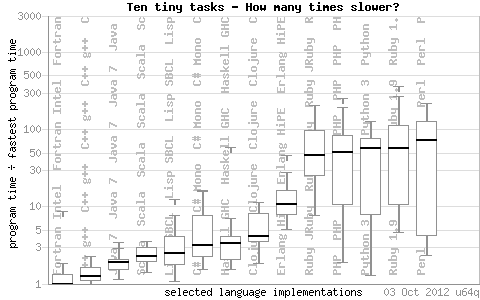
\includegraphics[scale=0.50]{CLshootout.png}
  \end{figure}
  \begin{itemize}
  \item From \href{http://shootout.alioth.debian.org/}{The Computer 
    Language Benchmarks Game (http://shootout.alioth.debian.org/)}
  \item Note logarithmic scale on program times
  \end{itemize}
\end{frame}

\begin{frame}{Good Performance 2}
  \begin{tabular}{lccccc}
     Slow
     &\begin{minipage}{0.625in}{\begin{figure}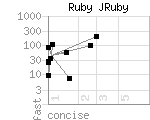
\includegraphics[scale=0.30]{jruby-CT.png}\end{figure}}\end{minipage}
     &\begin{minipage}{0.625in}{\begin{figure}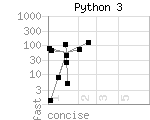
\includegraphics[scale=0.30]{python-CT.png}\end{figure}}\end{minipage}
     & \begin{minipage}{0.625in}{\begin{figure}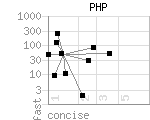
\includegraphics[scale=0.30]{php-CT.png}\end{figure}}\end{minipage}
     & &
\\
     Fast
     &&
     & \begin{minipage}{0.625in}{\begin{figure}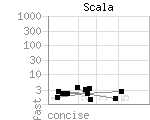
\includegraphics[scale=0.30]{scala-CT.png}\end{figure}}\end{minipage}
     & \begin{minipage}{0.625in}{\begin{figure}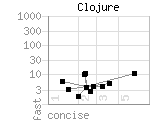
\includegraphics[scale=0.30]{clojure-CT.png}\end{figure}}\end{minipage}
     & \begin{minipage}{0.625in}{\begin{figure}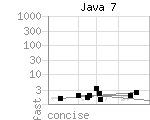
\includegraphics[scale=0.30]{java7-CT.png}\end{figure}}\end{minipage}
     \\
     & Concise & & & & Verbose
     \\
  \end{tabular}


  \begin{itemize}
  \item From \href{http://shootout.alioth.debian.org/}{The Computer 
    Language Benchmarks Game}
  \item Logarithmic scale on both axes
   \item Conciseness based on gziped size of benchmark program sources.
  \end{itemize}
  \note{}
 \end{frame}

\begin{frame}{Good Performance 3}
  \begin{itemize}
  \item Remember Little's Law $ N = A * T $
    \begin{itemize}
    \item $N$ -- the number of items in a system
    \item $A$ -- the average response time of the system
    \item $T$ -- the arrival rate of items
    \end{itemize}
  \item Reducing the average response time reduces the number of items
    in a system.
  \item Reducing the number of items reduces cost.
  \end{itemize}
  $ $\\
  $100 requests = 1.0 sec * 100 requests/sec$ \\
  $ $\\
  $ 10 requests = 0.10 sec * 100 requests/sec$ \\
\note{}
 \end{frame}

%% \section{The Scala Ecosystem}

\begin{frame}{The Scala Software Ecosystem}
  \begin{itemize}
  \item IDE Support
  \item Tools
  \item Frameworks
  \end{itemize}
  \note{}
\end{frame}



\begin{frame}{IDE Support}
  \begin{itemize}
  \item Scala has plugins (supports) for
    \begin{itemize}
    \item Eclipse
    \item IntelliJ
    \item NetBeans
    \end{itemize}
  \item Typesafe provides a version of Eclipse with a worksheet
  \end{itemize}
  \note{}
\end{frame}


\begin{frame}{Scala Tools}
  \begin{itemize}
  \item Simple Build Tool (sbt)
    \begin{itemize}
    \item Build tool for scala
    \item Uses Scala as a domain specific language to describe build process
    \item Works with Maven and Ivy repositories to resolve build and
      run-time dependencies.
  \end{itemize}
  \item Ensime for Emacs
    \begin{itemize}
    \item Provides 80\% of an IDE with Emacs editing capabilities
    \end{itemize}
  \end{itemize}
  \note{}
\end{frame}


\begin{frame}{Scala Frameworks - Lift}
  \begin{itemize}
  \item Lift Web provides an MVC-oriented framework for web applications
  \item Lift Web - applications are\footnote{From http://www.liftweb.net}
    \begin{itemize}
    \item Secure -- Lift apps are resistant to common vulnerabilities
      including many of the OWASP Top 10 
    \item Developer centric -- Lift apps are fast to build, concise and
       easy to maintain
     \item Designer friendly -- Lift apps can be developed in a totally
       designer friendly way 
     \item Scalable -- Lift apps are high performance and scale in the
       real world to handle insane traffic levels 
     \item Modular -- Lift apps can benefit from, easy to integrate, 
       pre-built modules
     \item Interactive like a desktop app -- Lift's Comet support is
       unparalleled and Lift's ajax support is super-easy and very
       secure
  \end{itemize}
  \end{itemize}
  \note{}
\end{frame}

\begin{frame}{Scala Frameworks - Akka}
  \begin{itemize}
  \item Expands Actors model to distributed systems
  \item Event-driven model
  \item Can scale to very large systems
  \item Provides a form of transactions
  \end{itemize}
  \note{}
\end{frame}


\begin{frame}{Scala Frameworks - Play}
  \begin{itemize}
  \item Provides a RESTful web application framework
  \item Based on MVC pattern.
  \item Uses Scala type system to provide high-performance
    type-checked templates  
  \item RDBMS support
  \end{itemize}
  \note{}
\end{frame}

%% \section{What makes Scala sizzle?}

\begin{frame}{What makes Scala sizzle}
  \begin{itemize}
  \item Scala works with existing Java and .NET code.
  \item There are no ''primitives'', every value is an Object.
  \item Every function is a value.
  \item Every value and expression have a type that can be statically checked.
  \item Scala can be extended with new operators.
  \item Implements both call-by-value and call-by-name conventions
  \item Pattern matching
  \item XML integration
  \item Actors for efficient concurrent objects
  \end{itemize}
\note{}
 \end{frame}

\begin{frame}[fragile]{Hello World!}
  \begin{tiny}
  \begin{verbatim}
object HelloWorld { def main(args: Array[String]) = println( "Hello World!")}
  \end{verbatim}
  or
  \begin{verbatim}
object HelloWorld { 
  def main(args: Array[String]) = println( "Hello World!")
}
  \end{verbatim}
  or
  \begin{verbatim}
object HelloWorld extends Application { println( "Hello World!") }
  \end{verbatim}
  runs thus:
  \begin{verbatim}
lthp01:code$ 
lthp01:code$ cat HelloWorld.scala
object HelloWorld { def main(args: Array[String]) = println( "Hello World!")}
lthp01:code$ scala HelloWorld.scala
Hello World!
lthp01:code$ 
  \end{verbatim}
  \end{tiny}
  \note{}
\end{frame}

\begin{frame}{Every value is an Object}
  \begin{itemize}
  \item No ``primitives''
  \item All operations are method calls\\
    {\tt  1 + 2 }\\

    is implemented as\\

    {\tt (1).+(2)}\\

    \item Syntactic ``sugar'' makes this bearable
  \end{itemize}
\note{}
 \end{frame}


\begin{frame}{Singleton Objects}
  \begin{itemize}
  \item Scala does not provide ``static'' objects for classes
  \item It provides singleton objects
  \end{itemize}
  \note{}
\end{frame}


\begin{frame}[fragile]{Singleton Object Example}
  \begin{tiny}
  \begin{verbatim}
 object HelloWorld extends Application { 
  val h = "Hello World!"
  def p( s : String ) = println(s )
  p(h)
}
  \end{verbatim}
  \end{tiny}
  \note{}
\end{frame}

\begin{frame}{Every function is a value}
  \begin{itemize}
  \item Scala is a functional programming language
  \item Scala supports closures and curried functions
  \item Functions can contain functions
  \end{itemize}
  \note{}
\end{frame}

\begin{frame}[fragile]{Closures}
  \begin{tiny}
  \begin{verbatim}
scala> var factor=4
factor: Int = 4

scala> val l = List(1, 2, 3 )
l: List[Int] = List(1, 2, 3)

scala> def multiply( x: Int ) = x * factor
multiply: (x: Int)Int

scala> multiply( 3 )
res0: Int = 12

scala> l.map( multiply )
res1: List[Int] = List(4, 8, 12)

scala> factor=5
factor: Int = 5

scala> l.map( multiply )
res2: List[Int] = List(5, 10, 15)
  \end{verbatim}
  \end{tiny}
\end{frame}
%scala>  :type multiply
%(x: Int)Int

\begin{frame}[fragile]{Curried Functions}
  \begin{tiny}
  \begin{verbatim}
scala> def mult(x: Int) (y: Int) = x * y
mult: (x: Int)(y: Int)Int

scala> l.map( mult(4))
res4: List[Int] = List(4, 8, 12)

scala> l.map( mult(factor))
res5: List[Int] = List(5, 10, 15)

scala> def cmult(x:Int) (y:Int) = x * y * factor
cmult: (x: Int)(y: Int)Int

scala> l.map(cmult(3))
res6: List[Int] = List(15, 30, 45)
  \end{verbatim}
  \end{tiny}
\end{frame}

\begin{frame}[fragile]{More fun with functions}
  \begin{tiny}
  \begin{verbatim}
scala> def f( i: Int ) = i + 7
f: (i: Int)Int

scala> def g( i: Int ) = i  * 3
g: (i: Int)Int

scala> def h( m: Int => Int, n : Int => Int, i : Int ) = m(n(i))
h: (m: Int => Int, n: Int => Int, i: Int)Int

scala> h(f, g, 5)
res1: Int = 22

scala> h(g, f, 5)
res2: Int = 36

scala> h( x => x + 22, g, 4)
res3: Int = 34

scala> h( x => x * 22, g, 4)
res4: Int = 264

scala> h( x => x * 22, x => x * 8, 4)
res5: Int = 704
  \end{verbatim}
  \end{tiny}
  \note{}
\end{frame}

\begin{frame}{Scala implements static type checking}
  \begin{itemize}
  \item Every expression has a type
  \item Eliminates many of run-time errors and checks
  \item Can infer the type of many expressions
  \end{itemize}
\note{}
 \end{frame}

\begin{frame}{Scala can be extended with new operators}
  \begin{itemize}
  \item Scala allows flexible names for methods (operators)
  \item Makes it easy to create new domain specific languages
  \end{itemize}
\note{}
 \end{frame}

\begin{frame}[fragile]{New operators, cont}
  \begin{tiny}
  \begin{verbatim}
case class WeirdInt( i: Int ) {
  def ?+ (j: WeirdInt) = WeirdInt( i + j.i )
  def ?- (j: WeirdInt) = WeirdInt( i - j.i )
  def ?* (j: WeirdInt) = WeirdInt( i * j.i )
  def ?/ (j: WeirdInt) = WeirdInt( i / j.i )
  def toInt = i
}
--
scala> :load WeirdInt.scala
Loading WeirdInt.scala...
defined class WeirdInt
scala> val z3=WeirdInt(3)
z3: WeirdInt = WeirdInt(3)
scala> val z5=WeirdInt(5)
z5: WeirdInt = WeirdInt(5)
scala> z3 ?* z5
res0: WeirdInt = WeirdInt(15)
scala> ( z3 ?* z5 ) + z5
<console>:12: error: type mismatch;
 found   : WeirdInt
 required: String
              ( z3 ?* z5 ) + z5
                             ^
scala> ( z3 ?* z5 ) ?+ z5
res2: WeirdInt = WeirdInt(20)
scala> z3 ?* z5 ?+ z5 toInt
res3: Int = 20
scala> (z3.?*(z5)).?+( z5).toInt
res4: Int = 20
  \end{verbatim}
  \end{tiny}
  \note{}
\end{frame}


\begin{frame}{Implements both call-by-value and call-by-name conventions}
  \begin{itemize}
  \item Call-by-value: evaluate function parameters, then call function
  \item Call-by-name: call function, let it decide whether it needs to
    evaluate its parameters
  \end{itemize}
  \note{}
\end{frame}

\begin{frame}[fragile]{Call By Value}
  \begin{tiny}
  \begin{verbatim}
scala> def cbv( a: Int, b: Int ) = if ( a < 5 ) a else b
cbv: (a: Int, b: Int)Int
scala> cbv( 3, 10 )
res14: Int = 3
scala> cbv( 7, 10 )
res15: Int = 10
scala> cbv( 3, 10/0 )
java.lang.ArithmeticException: / by zero
...
  \end{verbatim}
  \end{tiny}
  \note{}
\end{frame}

\begin{frame}[fragile]{Call By Name}
  \begin{tiny}
  \begin{verbatim}
scala> def cbv( a: Int, b: => Int ) = if ( a < 5 ) a else b
cbv: (a: Int, b: Int)Int
scala> cbv( 3, 10 )
res14: Int = 3
scala> cbv( 7, 10 )
res15: Int = 10
scala> cbv( 3, 10/0 )
res16: Int = 3
scala> cbv( 7, 10/0 )
java.lang.ArithmeticException: / by zero
...
  \end{verbatim}
  \end{tiny}
  \note{}
\end{frame}

\begin{frame}{Classes and Traits}
  \begin{itemize}
    \item Scala has single inheritance, just like Java
    \item Scala provides 'traits' to provide composition
    \item Traits similar to Java's interfaces, but more powerful
    \item Traits can include code, unlike Java's interfaces
    \item Classes provide the model for how to create objects
    \item Classes can be parametrized instead of explicit constructors
    \item Case classes provide syntactic sugar to
      \begin{itemize}
      \item provide factory methods
      \item implicitly make vals of fields
      \item permit pattern matching expressions on the class
      \end{itemize}
  \end{itemize}
  \note{}
\end{frame}

\begin{frame}[fragile]{Classes and Traits example}
  \begin{tiny}
  \begin{verbatim}
package examples
case class Person( firstName: String, lastName: String, age: Int )
trait USCitizen {
  private val myRep = Person( "Myke", "Representative", 45 )
  def representative = myRep
}
trait Senior { def ssOffice = "Unknown" }
case class USPerson( override val firstName: String,
		     override val lastName:  String,
		     override val age:       Int,
		                  ssn:       String )
     extends Person( firstName, lastName, age) with USCitizen
case class USSenior( override val firstName: String,
		     override val lastName:  String,
		     override val age:       Int,
		     override val ssn:       String ) 
     extends USPerson( firstName, lastName, age, ssn )
         with Senior
object ClassExample2 extends Application {
  val sally = Person( "Sally", "Simon", 20 )
  val billy = USPerson( "Billy", "Redmond", 30, "123-45-6789" )
  val mark  = USSenior( "Mark", "Miraldi", 66, "789-01-2345" )
  println( sally )
  println( billy )
  println( billy representative )
  println( mark )
  println( mark representative )
  println( mark ssOffice )
}
  \end{verbatim}
  \end{tiny}
  \note{}
\end{frame}

\begin{frame}[fragile]{Classes and Traits example execution}
  \begin{tiny}
  \begin{verbatim}
lthp01:code$ scala examples.ClassExample2
Person(Sally,Simon,20)
USPerson(Billy,Redmond,30,123-45-6789)
Person(Myke,Representative,45)
USSenior(Mark,Miraldi,66,789-01-2345)
Person(Myke,Representative,45)
Unknown
lthp01:code$ 
  \end{verbatim}
  \end{tiny}
  \note{}
\end{frame}

\begin{frame}[fragile]{Pattern Matching - Classes}
  \begin{tiny}
  \begin{verbatim}
// from from http://www.scala-lang.org/node/52
package examples

object patterns {
  abstract class Tree
  case class Branch(left: Tree, right: Tree) extends Tree
  case class Leaf(x: Int) extends Tree

  val tree1 = Branch(Branch(Leaf(1), Leaf(2)), Branch(Leaf(3), Leaf(4)))

  def sumLeaves(t: Tree): Int = t match {
    case Branch(l, r) => sumLeaves(l) + sumLeaves(r)
    case Leaf(x) => x
  }

  def toString(t: Tree): String = t match {
    case Branch(l, r) => "Branch(" + toString(l) + "," + toString(r) + ")"
    case Leaf(x)      => "Leaf(" + x + ")"
    }

  def main(args: Array[String]) {
    println("sum of leafs=" + sumLeaves(tree1))
    println("Tree: " + toString(tree1))
  }
}
Output:
lthp01:code$ scala examples.patterns
sum of leafs=10
Tree: Branch(Branch(Leaf(1),Leaf(2)),Branch(Leaf(3),Leaf(4)))
lthp01:code$ 
  \end{verbatim}
  \end{tiny}
  \note{}
\end{frame}


\begin{frame}{Scala and XML}
  \begin{itemize}
  \item Scala integrates XML into the language
  \item XML trees are just expressions
  \item Provides operators to search XML trees much like XPath
  \item Scala provides pattern matching for XML
  \end{itemize}
  \note{}
\end{frame}


\begin{frame}[fragile]{XML processing}
  \begin{tiny}
  \begin{verbatim}
case class Person( firstName: String, lastName: String, age: Int )

val sallyX = 
<Person>
<FName>Sally</FName>
<LName>Simon</LName>
<Age>20</Age>
</Person>

def XMLtoPerson( node: scala.xml.Node ) : Person =
   Person((node \  "FName").text,
	  (node \\ "LName").text,
	  (node \  "Age").text.toInt)

def personToXML(fname: String,
               lname: String,
	       age:   Int ) =
<Person>
<FName>{fname}</FName>
<LName>{lname}</LName>
<Age>{age}</Age>
</Person>

val sally = XMLtoPerson( sallyX )

val sallyX1 = personToXML( sally.firstName, sally.lastName, sally.age )
  \end{verbatim}
  \end{tiny}
  \note{}
\end{frame}


\begin{frame}[fragile]{XML code output}
  \begin{tiny}
  \begin{verbatim}
scala> :load xml-1.scala
Loading xml-1.scala...
defined class Person
sallyX: scala.xml.Elem = 
<Person>
<FName>Sally</FName>
<LName>Simon</LName>
<Age>20</Age>
</Person>
XMLtoPerson: (node: scala.xml.Node)Person
personToXML: (fname: String, lname: String, age: Int)scala.xml.Elem
sally: Person = Person(Sally,Simon,20)
sallyX1: scala.xml.Elem = 
<Person>
<FName>Sally</FName>
<LName>Simon</LName>
<Age>20</Age>
</Person>

scala> 
  \end{verbatim}
  \end{tiny}
  \note{}
\end{frame}

\begin{frame}{Actors}
  \begin{itemize}
  \item Actors provide a concurrency model
  \item Actors originated with the Erlang language
  \item An Actor provides a thread-like abstraction with a mailbox for messages
  \item Actors do not block, they run to completion
  \item Scala provides two functions for receiving messages:
    \begin{itemize}
    \item {\tt receive} - receive a message and return a result
    \item {\tt react} - receive a message and do not return a result
    \end{itemize}
  \item {\tt react} can be much more efficient than {\tt receive}
    since it doesn't have to return a result
  \item {\tt react} reuses threads to save setup/tear down time
  \end{itemize}
  \note{}
\end{frame}

\begin{frame}[fragile]{Actors (Ping Pong)}
    From http://www.scala-lang.org/node/54
  \begin{tiny}
  \begin{verbatim}
package examples.actors
import scala.actors.Actor
import scala.actors.Actor._

abstract class PingMessage
case object Start extends PingMessage
case object SendPing extends PingMessage
case object Pong extends PingMessage
abstract class PongMessage
case object Ping extends PongMessage
case object Stop extends PongMessage

object pingpong extends Application {
  val pong = new Pong
  val ping = new Ping(100000, pong)
  ping.start
  pong.start
  ping ! Start
}
  \end{verbatim}
  \end{tiny}
  \note{}
\end{frame}

\begin{frame}[fragile]{Actors (Ping)}
  \begin{tiny}
  \begin{verbatim}
class Ping(count: Int, pong: Actor) extends Actor {
  def act() {
    println("Ping: Initializing with count "+count+": "+pong)
    var pingsLeft = count
    loop {
      react {
        case Start =>
          println("Ping: starting.")
          pong ! Ping
          pingsLeft = pingsLeft - 1
        case SendPing =>
          pong ! Ping
          pingsLeft = pingsLeft - 1
        case Pong =>
          if (pingsLeft % 1000 == 0)
            println("Ping: pong from: "+sender)
          if (pingsLeft > 0)
            self ! SendPing
          else {
            println("Ping: Stop.")
            pong ! Stop
            exit('stop)
          }
      }
    }
  }
}
  \end{verbatim}
  \end{tiny}
  \note{}
\end{frame}

\begin{frame}[fragile]{Actors, (Pong)}
  \begin{tiny}
  \begin{verbatim}
class Pong extends Actor {
  def act() {
    var pongCount = 0
    loop {
      react {
        case Ping =>
          if (pongCount % 1000 == 0)
            println("Pong: ping "+pongCount+" from "+sender)
          sender ! Pong
          pongCount = pongCount + 1
        case Stop =>
          println("Pong: Stop.")
          exit('stop)
      }
    }
  }
}
  \end{verbatim}
  \end{tiny}
  \note{}
\end{frame}

\begin{frame}[fragile]{}
  \begin{tiny}
  \begin{verbatim}
lthp01:code$ scala examples.actors.pingpong
Ping: Initializing with count 10000: examples.actors.Pong@1f4384c2
Ping: starting.
Pong: ping 0 from examples.actors.Ping@19484a05
Ping: pong from: examples.actors.Pong@1f4384c2
Pong: ping 1000 from examples.actors.Ping@19484a05
Ping: pong from: examples.actors.Pong@1f4384c2
Pong: ping 2000 from examples.actors.Ping@19484a05
Ping: pong from: examples.actors.Pong@1f4384c2
Pong: ping 3000 from examples.actors.Ping@19484a05
Ping: pong from: examples.actors.Pong@1f4384c2
Pong: ping 4000 from examples.actors.Ping@19484a05
Ping: pong from: examples.actors.Pong@1f4384c2
Pong: ping 5000 from examples.actors.Ping@19484a05
Ping: pong from: examples.actors.Pong@1f4384c2
Pong: ping 6000 from examples.actors.Ping@19484a05
Ping: pong from: examples.actors.Pong@1f4384c2
Pong: ping 7000 from examples.actors.Ping@19484a05
Ping: pong from: examples.actors.Pong@1f4384c2
Pong: ping 8000 from examples.actors.Ping@19484a05
Ping: pong from: examples.actors.Pong@1f4384c2
Pong: ping 9000 from examples.actors.Ping@19484a05
Ping: pong from: examples.actors.Pong@1f4384c2
Ping: Stop.
Pong: Stop.
lthp01:code$ 
  \end{verbatim}
  \end{tiny}
  \note{}
\end{frame}


\begin{frame}{Resources}
  \begin{itemize}
  \item[] Web sites
    \begin{itemize}
    \item[] http://www.scala-lang.org  -- official Scala site
    \item[] http://www.scala-lang.org/api/current -- Scala API Documentation
    \item[] http://shootout.alioth.debian.org -- Computer language shootout 
    \end{itemize}
  \item[] Books
    \begin{itemize}
    \item[] {\it Programming in Scala, Second Edition}; Odersky,
      Spoon, Venners
    \item[] {\it Programming Scala}; Wampler, Payne; http://ofps.oreilly.com/titles/9780596155957/index.html
    \end{itemize}
  \item[] Tutorials and presentations
    \begin{itemize}
    \item[] http://www.slideshare.net/Odersky/fosdem-2009-1013261 --
      Scala - A scalable language
    \item[]http://www.slideshare.net/michael.galpin/introduction-to-scala-for-java-developers-presentation
      -- Scala for Java Developers
    \end{itemize}
  \end{itemize}
  \note{}
\end{frame}

\begin{frame}{Questions?}
  \note{}
\end{frame}

\end{document}


